\subsection{Traffic Demand Per Subscriber}\label{subsec:behavior}

Internet usage throughout a day follows diurnal sleep-patterns, and researchers
have shown that such patterns are in fact correlated with GDP, Internet 
allocations, as well as electrical consumption of 
a region~\cite{ant-diurnal-web}. This makes the study of usage behavior 
extremely relevant to the governmental bodies responsible
for development, such as the FCC, when considering policy decisions.

We start by evaluating traffic demand. We calculate demand by averaging the 
bytes transferred in uplink or downlink direction over the sample period (15 
minutes). This allows us to capture both the average per subscriber demand at 
any time in a day, and the aggregate demand at the ISP over a longer period, 
such as a day or a week.

To characterize the diurnal traffic demand observed at the ISP, we first 
calculate traffic demand per subscriber (table \ref{tab:eval-criteria}), and 
then plot the median and 95\%-ile of total usage over a week for both 
\treatment{} and \control{} sets (figure \ref{fig:TS-data-rate-daily}).

\begin{figure}[ht]
\begin{minipage}{\linewidth}
  \centering
  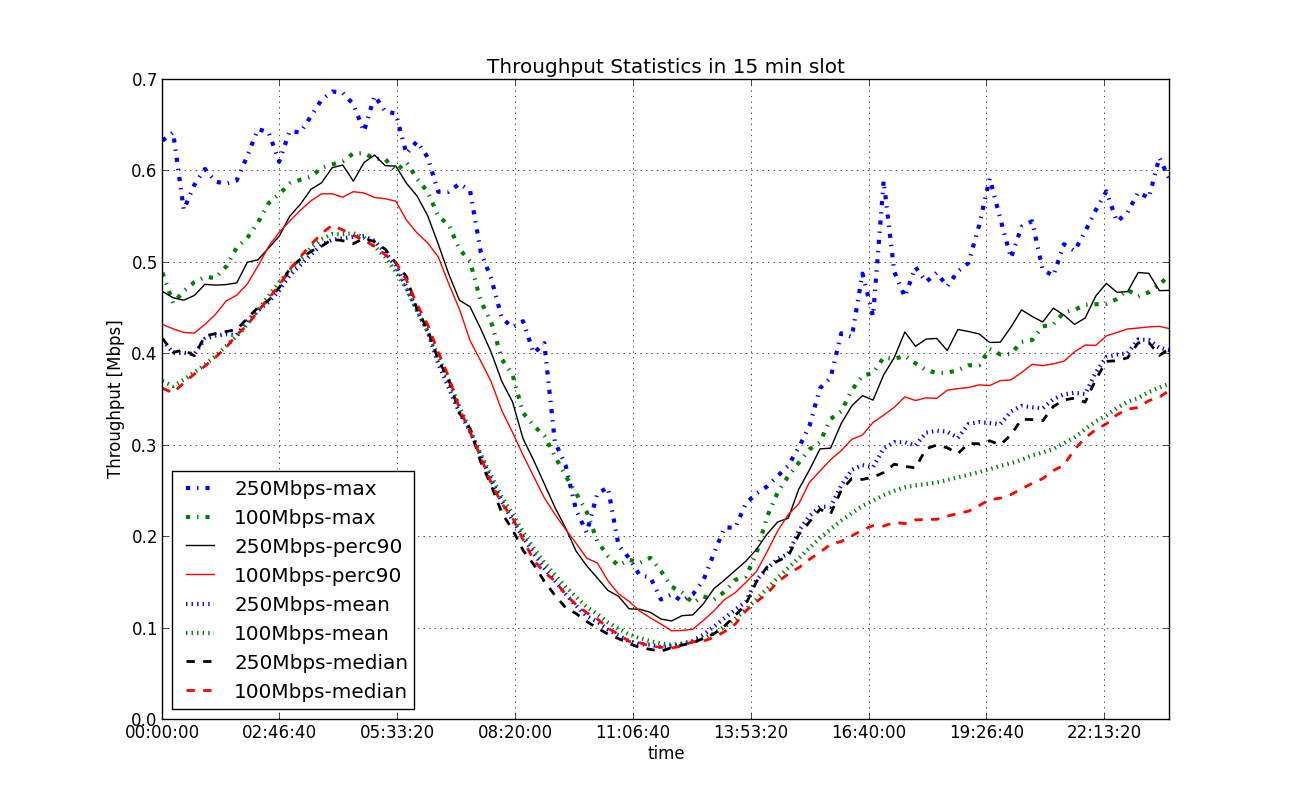
\includegraphics[width=\linewidth]{figures/describe-total-throughput-per-day[replace].png}
  \caption{agg (days) over means (devices): aggregate has no trough, peaks in the evening hours}
  %http://riverside.noise.gatech.edu:8083/separated/full/describe-total-throughput-per-day.png
  \label{fig:TS-data-rate-daily}
\end{minipage}
\end{figure}

Figure \ref{fig:TS-data-rate-daily} shows the aggregate data rate for a day. 
We observed that the median traffic demand during 7:00 PM -- 7:00 AM is 
\todo{XXX} for both \treatment{} and \control{}. However, during off peak 
daytime (work) hours, between 7:00 AM -- 7:00 PM, the \treatment{} group has a 
median of \todo{XXX}, 20\% higher than the \control{} set.

We observe that the rise to the peak prime time hour usage 
on weekdays is not plateaued like the pattern observed on weekends (and 
holidays). A generic (median) weekday aggregate usage consists of a rise in 
usage that starts early in the morning that builds up to the prime-time period, 
peaks, and then falls sharply. We do not observe a trough in mid afternoon 
(between 2:00 PM -- 6:00 PM), as is usually the case for overall usage observed 
at US Fixed access providers \cite{sandvine20141h}.


% EXPLAIN:
% LACK OF TROUGHS: users' behavior in higher tier bandwidth
% DISCREPANCY IN DAYTIME OFFPEAK: ???


\begin{figure*}[t]
\begin{minipage}{1\linewidth}
\centering
%
\begin{subfigure}[b]{0.3\linewidth}
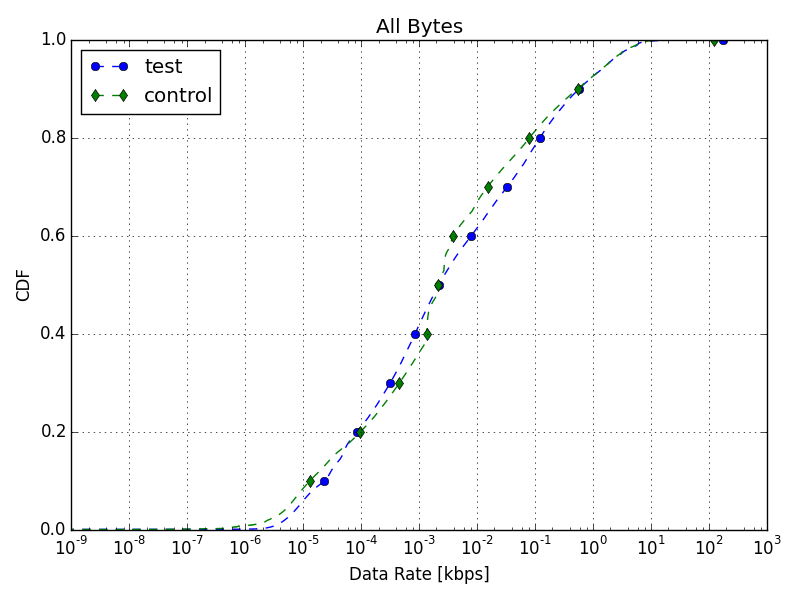
\includegraphics[width=\linewidth]{figures/cdf-all-bytes.png}
               \caption{for all devices}
\end{subfigure}
%
\begin{subfigure}[b]{0.3\linewidth}
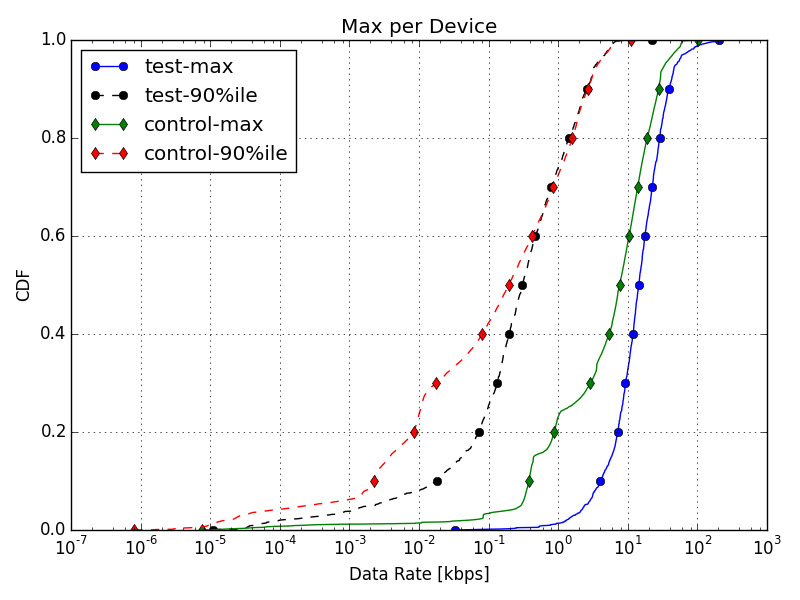
\includegraphics[width=\linewidth]{figures/cdf-max-per-device.png}
               \caption{CDF of max per device)}
\end{subfigure}
%
\begin{subfigure}[b]{0.39\linewidth}
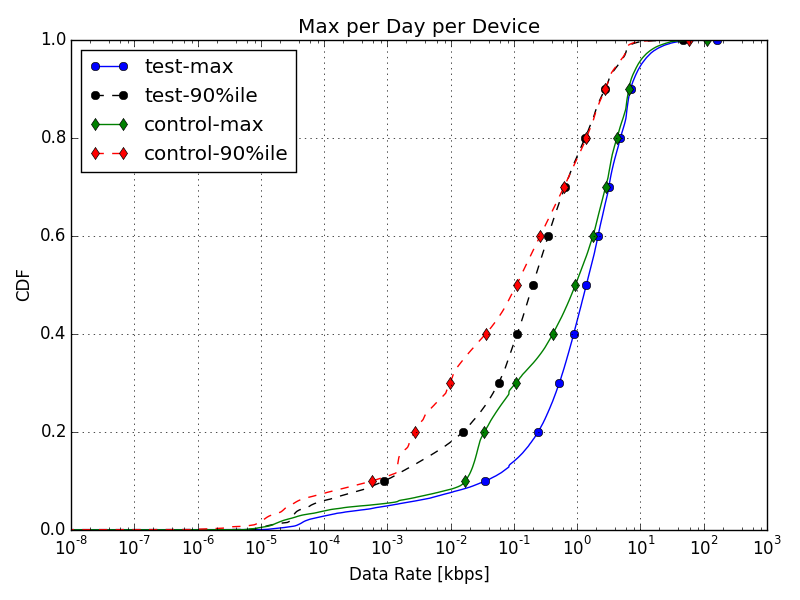
\includegraphics[width=\linewidth]{figures/cdf-max-per-day-per-device.png}
               \caption{Passive.\label{fig:tsval-passive}}
\end{subfigure}
%
\end{minipage}
\caption{Traffic Demand: The maximum data rate varies for test and control
103 set for low data rates, and this variation is present daily.}
\label{fig:tsval}
\end{figure*}



A comparison of the aggregate traffic demand distribution of all devices 
and sample periods shows that the \treatment{} has no significant affect on the 
mean traffic demand. 
